\chapter{Zarządzanie wielokomputerowym serwisem WWW}
\label{r04}
W rozdziale tym znajdzie się próba odpowiedzi na pytanie co to jest kiedy i po co stosuje się zarządzanie serwerem 
WWW (jakie są parametry charakterystyczne oceny wydajności i dostępności). Następnie zostanie przedstawiona szczegółowa 
taksonomia serwerów WWW. Ostatnim punktem tego rozdziału 
będzie porównanie usług zapewnianych przez witryny statyczne i dynamiczne, opis zastosowań i możliwości obu 
typów tworzenia witryn oraz wymagania stawiane systemom WWW wraz z poglądowym przykładem.

\section{Wprowadzenie}

Jak zauważono wcześniej -- przyszłość serwisów WWW należy do platform wieloserwerowych. Wynika to z możliwości 
teoretycznie niograniczonej rozbudowy wraz ze wzrostem liczby użytkowników oraz ich wymagań. Kolejną zaletą jest 
również spełnianie bezpieczeństwa przez takie wielokomputerowe systemy -- w dowolnym elemencie takiego systemu -- nodzie --
może nastąpić praktycznie dowolnego rodzaju uszkodzenie -- tak dysk, jak pamięć operacyjna czy procesor -- wtedy poszczególne
procesy są transportowane na inne nody, nawet w przypadku uszkodzenia jednej maszyny, nie spowoduje to przestoju. Jednakże aby
taki system spełniał dobrze swoje zadania potrzebne jest oprogramowanie lub urządzenie pozwające nim zarządzać czyli 
odpowiednio rozdysponować żądania klienckie oraz wykrywać uszkodzenia poszczególnych elementów układu. W literaturze
przyjęło się takie rozdysponowanie zapytań pomiędzy poszczególne nody nazywać równoważeniem obciążenia systemu\footnote{ang. 
\emph{load balancing, LB}}. 

\section{Równoważenie obciążenia -- metody}

Równoważenie obciążeń (ang. \emph{load balancing}) w systemach rozproszonych, to zagadnienie z dziedziny 
rozdziału zadań polegające na dystrybucji pomiędzy węzły systemu napływających do niego zleceń tak, aby  
maksymalizować jego łączną wydajność. Oznacza to, że działalność związana z rozdziałem zadań nie może powodować 
obciążenia systemu w stopniu, który niwelowałby korzyści wynikające z faktu zrównoważenia obciążeń jego węzłów. 
Angielski termin load balancing w rzeczywistości funkcjonuje jako reprezentant tej problematyki, gdyż traktowany 
ściśle oznacza doprowadzenie systemu rozproszonego do stanu w którym wszystkie jego węzły obciążone są w 
dokładnie równym stopniu, nawet jeżeli oznaczałoby to odebranie zadań jednemu z nich. W stosunku do większości 
rozwiązań przemysłowych z tego zakresu należałoby poprawnie używać określenia współdzielenie obciążeń (ang. \emph{
load sharing}) lub bardziej ogólnie, rozdział obciążeń (ang load distribution). Realizacja ścisłego równoważenia 
obciążeń wiąże się z koniecznością implementacji metod odbierania zadań węzłom, powoduje to wzrost złożoności 
realizacji algorytmu, a sam proces odbierania zadania jest dość kosztowny. Wzrost wydajności uzyskiwany dzięki 
idealnemu zrównoważeniu obciążeń w systemie w porównaniu do wydajności uzyskiwanej przy zastosowaniu 
współdzielenia obciążeń nie jest zwykle na tyle duży, by usprawiedliwiał ponoszenie kosztów związanych z 
pokonaniem złożoności realizacji ścisłego równoważenia obciążeń \cite{barylo13,barylo16,barylo17}. W tej pracy, tak jak w 
literaturze angielskojęzycznej, używany jest termin równoważenie obciążeń, chyba że zaznaczono inaczej.
Wydaje się, że najskuteczniejszą metodą zwiększenia wydajności serwera WWW jest powielenie (lub podział) danych, które 
serwer 
udostępnia, pomiędzy grupę połączonych siecią komputerów (dodatkowych serwerów WWW) i zapewnienie dostępu do 
tej grupy tak jak do pojedynczego serwera z uwzględnieniem transparentnego dla użytkownika i maksymalizującego 
wydajność podziału żądań HTTP pomiędzy poszczególne elementy grupy. Taka grupa nazywana klastrem lub farmą 
serwerów stanowi swoisty system rozproszony, którego wydajność można maksymalizować stosując równoważenie 
obciążeń. Należy zaznaczyć, że chociaż termin klaster oznacza serwery połączone w całość logiczną (dostępne pod 
jedną nazwą lub adresem IP), nie implikując żadnych ograniczeń na geograficzne rozproszenie serwerów, to wiele 
rozwiązań komercyjnych wymaga, by serwery należące do klastra znajdowały się w obszarze jednej sieci lokalnej 
(miały jednakową część globalną adresu IP).

\section{Przegląd i podział webowych algorytmów szeregowania}

Wszystkie mechanizmy realizujące zarządzanie dostępem do rozproszonych serwerów WWW muszą mieć zaimplementowany konkretny 
algorytm, na podstawie którego będą mogły podejmować decyzję o przesłaniu zapytania do najlepszego serwera. W zależności od 
stopnia skomplikowania systemu i możliwości implementacyjnych wykorzystywane algorytmy mogą mieć różną złożoność obliczeniową. 
Zastosowane strategie zależne są również od informacji, jakie posiada system na temat ilości zapytań generowanych przez 
klientów oraz informacji o stanie serwerów wchodzących w skład rozproszonego systemu WWW. Można je podzielić na kilka 
kategorii w zależności od ilości informacji, jaka wykorzystywana jest przy podejmowaniu decyzji. 

\subsection{Algorytmy statyczne (nie wykorzystujące informacji zewnętrznych)}
Jeżeli w procesie szeregowania nie są wykorzystywane żadne informacje o stanie serwerów lub strumieniu zapytań, mówi się o 
algorytmach statycznych. Te mechanizmy, to najprostsze rozwiązania gwarantujące w niewielkim stopniu rozłożenie obciążenia 
pomiędzy serwery. Rozkład ten jest bardzo przypadkowy i nie gwarantuje równomiernego wykorzystania zasobów ani wysokiej 
dostępności systemu, jednakże są one najszybszymi, gdyż wymagają najmniej mocy obliczeniowej. Do takich algorytmów należą:
\begin{itemize}
\item Random -- system nie posiada żadnych informacji o stanie serwerów WWW, jak również nie posiada informacji o tym, do 
którego serwera ostatnio skierowane zostało zapytanie;
\item Round--robin -- system nie posiada żadnych informacji o stanie serwerów WWW, posiada jednak informację historyczną o tym, 
do którego serwera skierowane zostało ostatnio nadesłane zapytanie.
\end{itemize}

\subsection{Algorytmy dynamiczne (wykorzystujące informację zewnętrzną)}
W procesie szeregowania można stosować bardziej rozbudowane mechanizmy zarządzania. Aby zwiększyć efektywność szeregowania, 
można stosować strategie wykorzystujące informacje o kliencie. Wybór najlepszego serwera może odbywać się na podstawie adresu 
IP lub numer portu TCP wykorzystywanego przez klienta. Możliwe jest również wykorzystywanie tzw. alarmów generowanych przez 
serwery. Do mechanizmu decydującego o wyborze serwera w określonych odstępach czasowych przekazywana jest informacja zwrotna o 
obciążeniu serwera lub informacja o przekroczeniu jakiegoś określonego parametru. Szeregowanie może odbywać się na podstawie 
jednej z metryk określających obciążenie:
\begin{itemize}
\item ilości aktywnych połączeń z serwerem,
\item wykorzystania dysku i/lub procesora serwera,
\item przewidywanego strumienia zapytań w określonym czasie.
\end{itemize}

W przypadku modeli, gdzie mechanizmy szeregowania w całości kontrolują strumień zapytań, mogą być stosowane algorytmy 
dystrybuujące zapytania w zależności od wielkości napływającego strumienia oraz obciążenia serwerów obsługujących te 
zapytania. Dzięki informacjom zbieranym od serwerów możliwe jest szacowanie parametrów mających wpływ na szybkość ich 
odpowiedzi. Mogą to być:
\begin{itemize}
\item ilość zapytań zrealizowana w określonym czasie,
\item obciążenie procesora w danym momencie,
\item poziom wykorzystania dysków w serwerze.
\end{itemize}
Takie rozwiązania umożliwiają wyeliminowanie przeciążonych serwerów. W znacznym stopniu zwiększa to dostępność klientów do 
danych oraz wpływa na lepsze wykorzystanie zasobów. 

Algorytmy dynamiczne możemy w zależności od miejsca analizy podzielić na:
\begin{itemize}
\item \emph{Server Info Aware} -- czyli wykorzystujące informacje o stanie serwera;
\item \emph{Client Info Aware} -- czyli wykorzystujące specyfikę żądań klienckich -- przekierowujące żądania w zależności
od typu zapytania klienckiego (dane z serwera baz danych, wykorzystujące skrypty CGI, zawierające pliki multimedialne itp.)
\end{itemize}

\subsection{Algorytmy szeregowania wykorzystywane po stronie serwera DNS}

\subsubsection{Algorytmy nie wykorzystujące informacji o stanie systemu -- statyczne}

\begin{itemize}
\item Round--robin DNS\\
Podejście to zostało zastosowane jako pierwsze przy budowie skalowalnego systemu serwerów webowych przez NCSA \cite{modele22}. Kod 
serwera DNS (np. Unixowy BIND) bez żadnych modyfikacji może wykorzystywać algorytm Round--robin. Obciążenie serwerów nie jest 
zbyt dobrze 
równoważone ze względu na mechanizm cache dla powiązań nazwa domenowa - adres IP. Stosując takie podejście, nie ma się również 
kontroli nad dostępnością serwerów oraz nie uwzględnia się możliwości zastosowania serwerów o różnej wydajności.
Jest to algorytm bardzo prosty zarówno w działaniu jak i implementacji (w stadardowym serwerze DNS można go zastosować, bez
konieczności modyfikacji kodu serwera). Jego działanie polega na cyklicznym rozsyłaniu pakietów do kolejnego na liście serwera.
Oczywiście najlepsze wyniki osiąga się dla komputerów symetrycznych sprzętowo. Modyfikacją tego algorytmu jest 
Weighted Round--Robin, w którym to algorytmie można statycznie nadać wagi poszczególnym serwerom w zależności od ich 
wydolności;
\item Random\\
\end{itemize}

\subsubsection{Algorytmy wykorzystujące informacje o stanie systemu}

Alternatywą dla algorytmu Round--robin najczęściej stosowanego w przypadku serwera DNS są algorytmy wykorzystujące informacje o 
stanie systemu (wielkości przewidywanego strumienia zapytań, aktualnego obciążenia serwerów). Okazuje się, że reguły bazujące 
wyłącznie na stanie obciążenia serwerów WWW są nieefektywne. W rzeczywistości, w związku z hierarchicznym buforowaniem danych 
przez serwery DNS, pojedyncze zapytanie od klienta może spowodować napływ wielu innych zapytań. Wynika z tego, że informacja o 
aktualnym obciążeniu nie jest w żaden sposób związana z przyszłym obciążeniem \cite{ModeleFunkcjonalne}.
Podejście pozwalające oszacować nadchodzący strumień zapytań (\emph{hidden load weight}) w czasie TTL (\emph{Time To Live}) jest najbardziej 
efektywne. Dzięki tym informacjom można przypisać różne wartości TTL dla różnych domen i estymować wielkość ukrytego, czyli 
niekontrolowanego przez serwer DNS strumienia zapytań. Przykładami tego typu algorytmów są \cite{modele14}:
\begin{itemize}
\item Multi tie round--robin -- dla każdej domeny lub ich określonych zbiorów przypisywane są różne wartości TTL, pozwalające na
zrównoważenie strumieni zapytań do każdego serwera WWW.
\item Dynamically accumulated load (DAL) -- rozbudowana wersja algorytmu Multi tie Round--robin polegająca na zbieraniu 
informacji o estymowanej wielkości obciążenia serwerów i zmianie łańcucha przypisań adresów w serwerze DNS w zależności od 
zakładanego obciążenia.
\item Minimum residual load -- modyfikacja algorytmu DAL polegająca na estymowaniu wielkości ukrytego obciążenia i wartości TTL.
Po upływie TTL serwer WWW odpytywany jest o rzeczywistą wielkość strumienia zapytań, jaka została do niego skierowana. Dzięki 
temu algorytm ma informację o stanie serwera. Powoduje to również zmianę kolejności przypisań w serwerze DNS;
\end{itemize}

\subsubsection{Algorytmy adaptacyjne}

Algorytmy równoważenia bazujące na oszacowaniu hidden load weight oraz alarmach z krytycznie przeciążonych serwerów pozwalają 
na dużo bardziej efektywne, w porównaniu z algorytmami Round--robin, równoważenie serwerów WWW. Niestety, są one efektywne 
tylko w przypadku rozproszenia serwerów homogenicznych. Inną grupą algorytmów przeznaczonych do równoważenia obciążenia 
serwerów heterogenicznych są algorytmy adaptacyjne. W przypadku algorytmów adaptacyjnych wartość TTL przypisywana jest 
dynamicznie do każdego żądania na podstawie przewidywanego hidden load weight oraz wydajności serwera, do którego zapytanie 
zostało przypisane. Idea tego podejścia polega na uwzględnieniu pewnej wartości $\xi_i$ opisującej moc obliczeniową serwera $S_i$. 

Algorytmy te podzielone zostały na dwie grupy \cite{modele25}:
\begin{itemize}
\item probabilistyczne -- realizacja metody bazuje na algorytmie Round--robin. Za każdym razem losowo generujemy liczbę 
$\gamma(0\leq\gamma\leq1)$. Jeżeli zapytania przypisane są aktualnie do serwera $S_i$, to jako następny zostanie 
wybrany $S_{i+1}$ tylko wtedy,
gdy $\gamma\leq\xi_i$, w przeciwnym przypadku warunek zostaje rozpatrzony dla kolejnego serwera. 
Wartość TTL oblicza się ze wzoru:
\begin{equation}
TTL_i = \frac{\eta}{\xi_i}
\end{equation}
\item deterministyczne -- ideą algorytmu jest takie dostosowanie czasu TTL, aby bardziej wydajne serwery obsługiwały więcej 
zapytań, a mniej wydajne nie były przeciążane. Dla każdej domeny $i$ obsługiwanej przez system serwerów webowych zostaje 
przypisana wartość TTL z  uwzględnieniem wydajności serwera $j$ według wzoru:
\begin{equation}
TTL_{ij} = \frac{\eta * c_i}{\xi_i}
\end{equation}
gdzie $\eta$ jest wartością stałą, zależną od liczby zdefiniowanych domen generujących zapytania.
\end{itemize}

\subsection{Algorytmy szeregowania wykorzystywane w dystrybutorach}

Stosowane tutaj algorytmy  \cite{modele13} są najprostsze, ponieważ dystrybutor obsługuje wszystkie nadchodzące pakiety i konieczne jest 
zminimalizowanie czasu poświęcanego na ich obsługę. Rekompensatą za konieczność obsługi wszystkich pakietów jest pełna 
kontrola napływającego strumienia zapytań. Stosowane w tym przypadku algorytmy można podzielić na trzy podstawowe grupy:
\begin{itemize}
\item Information less -- nie wykorzystujące żadnych informacji o stanie systemu,
\item Client info aware -- wykorzystujące informacje o adresie IP klienta lub numerze portu, przez który komunikuje się z 
serwerem,
\item Server state aware -- wykorzystujące informacje o stanie serwera, do którego przekazują zapytanie.
\end{itemize}

Tak jak w przypadku algorytmów stosowanych w serwerze DNS, najmniej efektywne są algorytmy nie wykorzystujące żadnych 
dodatkowych informacji, czyli Random i Round--robin.

Wykorzystując informacje o kliencie, np. jego adres IP, można zastosować bardziej efektywne rozwiązania. Przykładem takiego 
algorytmu jest Client partition.

W związku z zarządzaniem strumieniem zapytań na poziomie pakietów, odwołania nadchodzące z tego samego adresu, dotyczące 
pojedynczej sesji, muszą być przekierowywane do tego samego serwera. Dopiero żądania nowego obiektu mogą być przesłane na inny 
serwer. Wymaga to utrzymywania w systemie tablicy aktywnych połączeń. Dzięki temu można oszacować, który z serwerów obciążony 
będzie dodatkowymi zapytaniami w najbliższym czasie i na tej podstawie wybrać najlepszy, do którego skierowane zostanie 
kolejne zapytanie. Realizowane jest to na podstawie algorytmu Least loaded server. 
\begin{figure}[h]
\centering
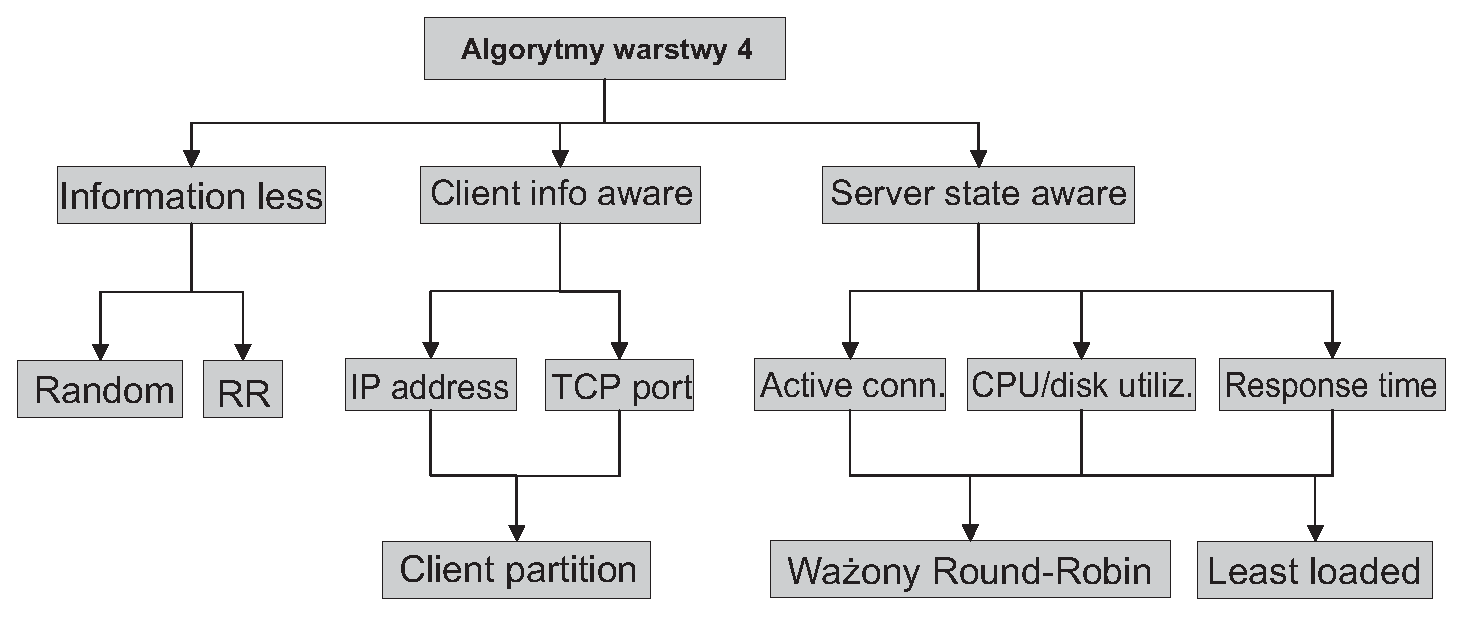
\includegraphics[width=4.9in]{./rysunki/level_4_alg.eps}
\caption{Algorytmy stosowane w dystrybutorach.}
\label{level_4_alg}
\end{figure}

Oprócz informacji o tym, kto przesyła zapytania do systemu webowego, można również uzyskać dane na temat pracy poszczególnych 
serwerów w systemie. Aby poprawić jakość szeregowania zapytań, w algorytmie dokonującym wyboru najlepszego serwera stosuje się 
różnego rodzaju metryki określające aktualne obciążenie serwerów. Najczęściej stosowanymi algorytmami w tym przypadku są Least 
loaded server oraz Weighted Round--robin. 
\begin{itemize}
\item W przypadku algorytmu Least loaded server dzięki wybranemu kryterium (określonej metryce) wiemy, który z serwerów 
powinien przyjąć kolejne zapytanie. Odbywa się to na zasadzie: najmniej obciążony serwer przyjmuje kolejne zlecenie. 
\item Stosując algorytm Weighted Round--robin, przy wyborze kolejnego serwera można uwzględniać metrykę jako parametr funkcji 
wyboru najlepszego serwera.

Ważnym więc elementem funkcjonowania tego rozwiązania jest dobór metryki będącej powyższym parametrem. Istnieje 
możliwość kontrolowania następujących parametrów:
\begin{itemize}
\item input metric -- informacja pozyskiwana jest przez dystrybutor bez współprcy z serwerami, np. liczba aktywnych połączeń 
miedzy dystrybutorem a poszczególnymi serwerami,
\item server metric -- informacja pozyskiwana jest przez serwery i dostarczana dystrybutorowi, np. wykorzystanie procesora lub 
dysku, czas miedzy otrzymaniem zapytania a wysłaniem odpowiedzi,
\item forward metric -- informacja pozyskiwana jest bezpośrednio przez dystrybutor, np. emulacja zapytań do serwerów webowych.
\end{itemize}
\end{itemize}

\subsection{Algorytmy szeregowania wykorzystywane w przełącznikach webowych}
Przełączniki webowe mają również możliwość kontrolowania 100\% ruchu do serwerów. Zatem i tu konieczne jest wykorzystanie jak 
najprostszych mechanizmów zarządzania. W przypadku prostych rozwiązań wystarczająco wydajne są algorytmy statyczne. Sytuacja 
taka występuje, gdy czasy realizacji zleceń przez serwery WWW są bardzo zbliżone do siebie i nie wychodzą poza określony 
przedział wartości.

W przypadku gdy w systemie występują więcej niż dwa ograniczenia czasu obsługi zlecenia, należy stosować algorytmy dynamiczne 
wykorzystujące informacje o kliencie lub stanie serwera (client info or server state aware). Mając do dyspozycji 
heterogeniczne środowisko serwerów trudno jest wybrać najlepszy, wspólny dla wszystkich parametr określający metrykę 
obciążenia serwera. W takim przypadku preferowane są algorytmy wykorzystujące informacje pochodzące od klientów.
\begin{figure}[h]
\centering
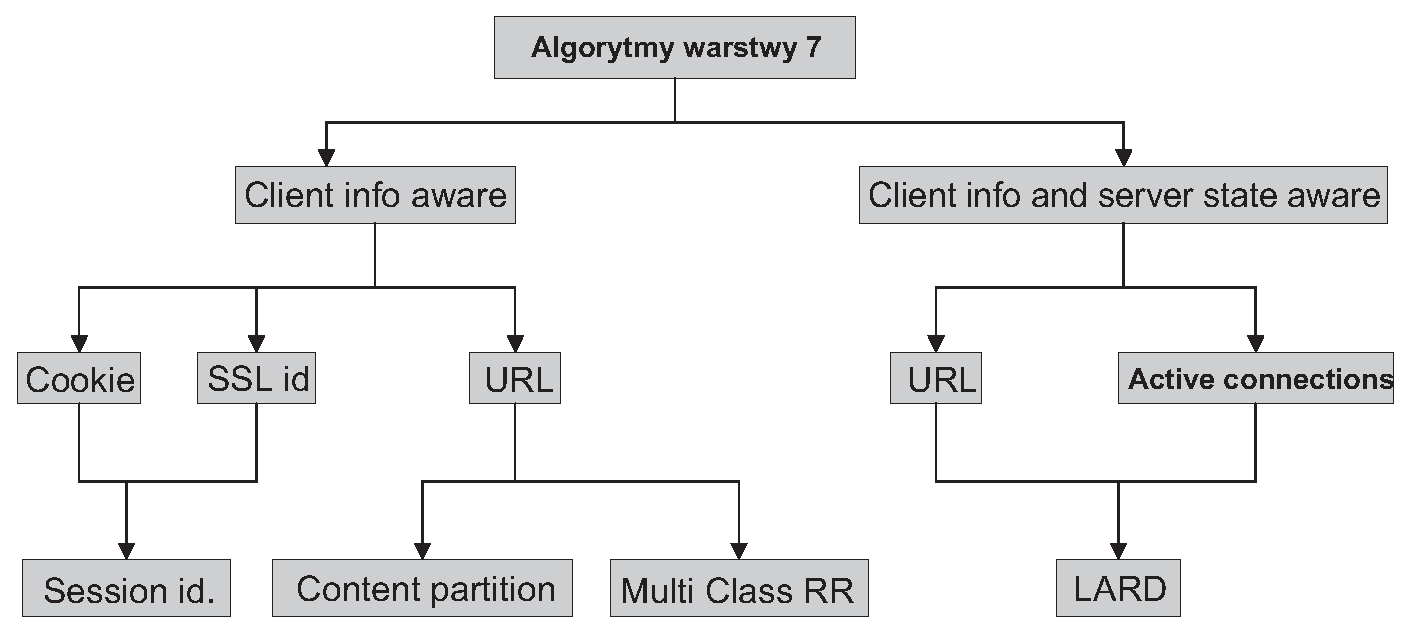
\includegraphics[width=4.9in]{./rysunki/level_7_alg.eps}
\caption{Algorytmy stosowane w przełącznikach webowych.}
\label{level_7_alg}
\end{figure}

Jak wynika z rysunku \ref{level_7_alg}, istnieją trzy rodzaje algorytmów opartych na informacjach o kliencie:
\begin{itemize}
\item Session identifiers -- odwołania HTTP, mające ten sam identyfikator SSL lub ten sam znacznik cookie przypisywane są do 
tego samego serwera -- zmniejsza to czas konieczny na ponowną identyfikację klienta,
\item Content partition -- podział zasobów serwerów może nastąpić ze względu na:
\begin{itemize}
\item typy plików -- dane, pliki graficzne, pliki audio umieszczone są na specjalizowanych serwerach,
\item wielkość plików -- duże pliki na szybszych serwerach lub równomierne rozłożenie plików w przypadku serwerów 
homogenicznych, 
\end{itemize}
\item Multi--class round--robin -- zasoby są podzielone ze względu na złożoność obliczeniową i czasową, jaka zostanie 
wygenerowana podczas ich obsługi, np. połączenia szyfrowane wymagają mocy obliczeniowej procesora, odwołania do bazy danych 
wymagają zwiększonej obsługi dysków, czy wreszcie pobieranie dużych plików w znacznym stopniu obciąża sieć.
\end{itemize}

Zasada działania algorytmu wykorzystującego informacje o kliencie i serwerze jest następująca. Pierwsze zapytanie klienta o 
zasoby przekierowywane jest według algorytmu Least loaded server (metryką jest ilość aktywnych połączeń z serwerem). Pozostałe 
zapytania klienta o ten sam zasób przekierowywane są do tego samego serwera. Dzięki temu zwiększona jest skuteczność odwołań 
do pamięci podręcznej (cache) tego serwera. Algorytm ten zwany jest Locality-Aware Request Distribution (LARD).

\subsection{Algorytmy szeregowania wykorzystywane w przypadku przekierowań na poziomie protokołu HTTP}

Gdy stosuje się rozwiązania oparte na warstwowej strukturze, istnieje możliwość zarządzania zapytaniami z poziomu protokołu \cite{modele18}. 
Takie rozwiązanie jest przezroczyste dla użytkowników. Głównym celem stosowania tego mechanizmu jest zapobieganie 
przeciążeniom serwerów webowych. Przekierowywanie odbywa się poprzez przesłanie klientowi informacji w nagłówku: HTTP OK. 
302 -- Moved temporary to a new location.

Adres nowej lokalizacji może być podany w postaci nazwy domenowej lub adresu IP. Podanie adresu IP jest bardziej efektywne, 
ponieważ następuje bezpośrednie odwołanie do nowego serwera (klastra), a nie do serwera DNS.
Przekierowania można realizować w zależności od kilku parametrów \cite{modele13}. Proces przekierowań może dotyczyć:
\begin{itemize}
\item wszystkich stron,
\item tylko stron przekraczających określoną wielkość,
\item tylko stron, których ilość obiektów składowych przekracza określoną liczbę,
\end{itemize}

Wybór serwera, który powinien przejąć zapytanie, może odbywać się z wykorzystaniem jednej z poniższych strategii:
\begin{itemize}
\item Round--robin,
\item Least Loaded,
\item Hash function,
\item Client to server proximity.
\end{itemize}

\section{Metody równoważenia obciążeń -- przykłady}

\subsubsection{Równoważenie obciążeń z wykorzystaniem filtra datagramów}

Inną implementacją rozproszonego algorytmu współdzielenia obciążeń jest zastosowanie na każdym serwerze 
wchodzącym w skład klastra tzw. filtra datagramów. Klaster taki powinien być połączony z Internetem poprzez 
pojedynczy router brzegowy. Każdy serwer w klastrze posiada skonfigurowane dwa adresy IP: adres ,,prywatny'' i 
jednakowy dla wszystkich serwerów adres IP klastra. Router po otrzymaniu datagramu opatrzonego adresem IP 
klastra nadaje mu fizyczny (sprzętowy np. adres Ethernet) adres typu broadcast (jeżeli do routera przyłączone 
są tylko serwery należące do klastra) lub multicast (jeżeli klaster jest tylko wyróżnioną grupą wśród 
wszystkich hostów przyłączonych do serwera). Zastosowanie takiego adresu sprawia, że karty sieciowe wszystkich 
serwerów w klastrze akceptują datagram. Pomiędzy sterownikiem karty sieciowej, a oprogramowaniem TCP/IP na 
każdym serwerze musi pracować specjalny proces, który zadecyduje, czy pakiet należy odrzucić czy obsłużyć. 
Proces ten nazywamy filtrem pakietów \cite{barylo34}. Decyzja o odrzuceniu lub obsłużeniu datagramu podejmowana jest na 
podstawie zawartości dwóch struktur danych: tablicy połączeń TCP (datagramy należące do jednego połączenia 
TCP muszą być obsługiwane przez serwer który nawiązał dane połączenie) oraz tablicy zawierających wielkość 
obciążenia poszczególnych serwerów klastra. Tablica ta jest uaktualniana przez same serwery. Każdy serwer musi 
wysyłać okresowo komunikat typu broadcast zawierający wielkość jego obciążenia. Jeżeli do klastra nadchodzi 
datagram otwierający nowe połączenie TCP (nagłówek TCP zawiera flagę SYN) serwer o najniższym indeksie 
obciążenia w tablicy (indeksem tym jest zwykle liczba otwartych połączeń TCP) jest zobowiązany do jego 
przyjęcia. Dla zwiększenia wydajności klastra w serwerach stosować można dwie karty sieciowe: jedną ze 
skonfigurowanym adresem IP klastra i drugą z prywatnym adresem serwera.  W takim przypadku pakiety, które nie 
muszą być filtrowane (np. wymiana danych SNMP) przechodzić będą przez  ,,prywatną'' kartę. Ten typ równoważenia 
dotyczyć może każdej usługi korzystającej z TCP, w szczególności WWW.
Pierwszą komercyjną implementacją tego rozwiązania był pakiet oprogramowania Convoy Cluster firmy 
Valence Research przeznaczony dla systemu Microsoft Windows NT. Jako miarę obciążenia serwera przyjęto w nim 
ilość otwartych połączeń TCP, a komunikaty ogłaszające stan obciążenia wysyłane były przez serwery co sekundę. 
Oprogramowanie umożliwiało dynamiczną konfigurację klastra przez dodawanie lub usuwanie serwera z klastra bez 
przerywania pracy klastra. Serwery w klastrze musiały powielać swoje dane. W pierwszej wersji wymagane było 
stosowanie dwóch kart sieciowych na każdym serwerze, a nadchodzące datagramy rozgłaszane były w trybie broadcast 
(docierały do każdego hosta w sieci lokalnej klastra, nawet jeśli nie był on serwerem) Wersja 2.0 Convoy 
Cluster wyeliminowała te niedogodności i oferowała liczne dodatkowe możliwości konfiguracyjne np. opcjonalne 
stosowanie pokrewieństwa z klientem (ang. \emph{client affinity}), co umożliwia obsługę wszystkich datagramów 
nadchodzących od raz zidentyfikowanego (w trakcie nawiązywania pierwszego połączenia) klienta przez jeden 
serwer. W roku 1999 firma Microsoft wykupiła od Valence Research technologię Convoy Cluster i po 
,,kosmetycznych'' zmianach udostępniła ją w pakiecie Microsoft Windows NT 4.0 Enterprise Server pod nazwą 
Microsoft Load Balancing Service.
Najważniejszą zaletą stosowania filtra pakietów jest jego duża wydajność w porównaniu do 
scentralizowanych urządzeń rozdzielających zadania (np. LSNAT). Uzyskiwane jest to dzięki temu, że na żadnym 
etapie obsługi zadania nie są modyfikowane datagramy i nie istnieje pojedynczy punkt podejmowania decyzji o 
obsłudze zadania. Ważna jest również łatwość konfiguracji klastra i duża niezawodność (serwer, który ulega 
awarii przestaje wysyłać komunikaty o stanie swego obciążenia, nie jest więc uwzględniany w tablicach obciążenia 
serwerów w pozostałych węzłach klastra i w ten sposób nie bierze udziału w równoważeniu obciążeń). Koszt jaki 
należy ponieść, aby uzyskać te niewątpliwie pożądane cechy to trudniejsza konfiguracja poszczególnych serwerów 
(konieczność instalacji i konfiguracji filtra pakietów) oraz duży ruch w sieci lokalnej klastra wynikający z 
aktualizacji tablic obciążenia. Aktualizacje te muszą być częste, gdyż łatwo można wyobrazić sobie sytuację, w 
której serwer o najniższym indeksie obciążenia ulega awarii. W takiej sytuacji pozostałe serwery aż do 
aktualizacji swoich tablic obciążenia będą odrzucać wszystkie datagramy otwierające nowe połączenia, co z 
pewnością nie jest zjawiskiem pożądanym.

\subsubsection{Równoważenie obciążeń z wykorzystaniem redirekcji HTTP}

Redirekcja jest  mechanizmem protokołu HTTP, który zaprojektowano z myślą o obsłudze sytuacji w których 
zasób (plik) wskazywany przez pewien URL zmienia swoje fizyczne położenie (zostaje przeniesiony na inny serwer) 
i w związku z tym uzyskuje inny URL. Aby nie zmuszać użytkownika do poszukiwania tego zasobu na własną rękę 
serwer WWW przechowuje tzw. tablice redirekcji. Jest to tablica zawierająca URL, które wcześniej dotyczyły 
zasobów danego serwera, lecz obecnie zasoby te znajdują się pod innym URL. Tablica zawiera również aktualny URL 
dla każdego przeniesionego zasobu. W przypadku zapytania o taki ,,zdezaktualizowany'' URL serwer WWW zwraca 
odpowiedź HTTP typu ,,przeniesiono'' i jako dane przekazuje aktualny URL zasobu. Przeglądarka po otrzymaniu takiej 
odpowiedzi musi zestawić nowe połączenie z serwerem wskazanym przez otrzymany URL.

Opisany mechanizm w prosty sposób wykorzystać można do pewnego rodzaju równoważenia obciążeń serwerów 
WWW \cite{barylo22,barylo23}. W klastrze serwerów wydzielić można tzw. serwer redirekcji, którego nazwa DNS reprezentować 
będzie cały klaster. Jedynym zadaniem takiego serwera jest utrzymywanie tablicy redirekcji i przekierowanie 
nadchodzących zapytań do odpowiedniego serwera z klastra. W takiej architekturze serwery zwykle nie powielają 
swych zasobów, każdy z nich przechowuje część danych udostępnianych przez klaster, a to który z nich obsłuży 
zapytanie determinowane jest przez rodzaj żądanych informacji. Przykładowo jeśli pod nazwą www.pogoda.com 
dostępny jest serwis prezentujący prognozę pogody dla każdego kontynentu to zasoby serwisu podzielić można 
pomiędzy siedem serwerów (po jednym dla każdego kontynentu) a pod adresem IP stanowiącym odwzorowanie nazwy 
serwisu należy umieścić serwer redirekcji. W odpowiedzi na zapytanie o dowolny URL zaczynający się np. od ciągu 
www.pogoda.com/Azja/ serwer redirekcji dokonywałby przekierowania do serwera przechowującego dokumenty o 
pogodzie w Azji (np. wwwazja.pogoda.com) \cite{barylo22}. Poniższy rysunek przedstawia schemat nawiązywania 
połączenia w przypadku stosowania redirekcji HTTP:
\begin{figure}[h]
\centering
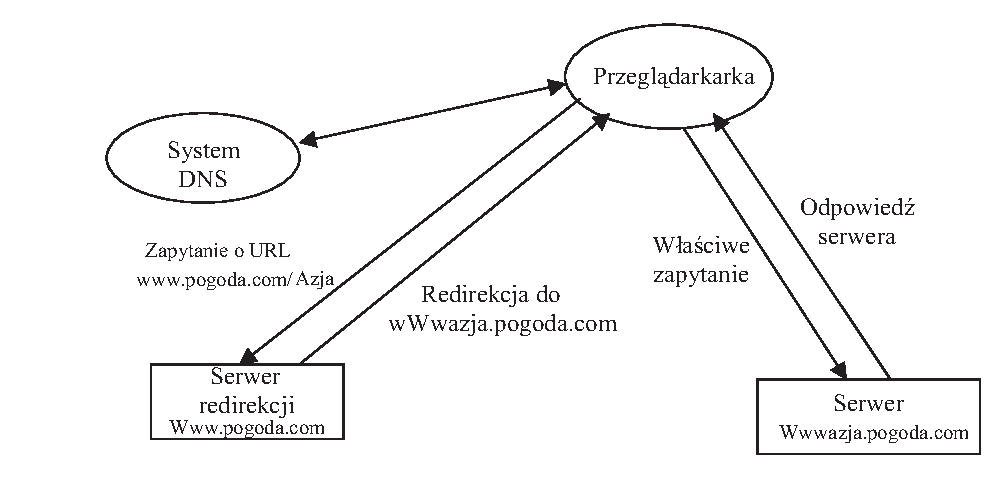
\includegraphics[width=4.9in]{./rysunki/redirekcja.eps}
\caption{Schemat redirekcji HTTP.}
\label{redirekcja}
\end{figure}

Stosowanie redirekcji ma zasadniczo dwie zalety. Po pierwsze utrzymanie statycznej tablicy redirekcji jest 
bardzo proste i tanie w implementacji, nie wymaga stosowania specjalnego sprzętu ani oprogramowania. Po drugie, 
ponieważ używane są adresy URL, klaster stanowiący logiczną całość może być rozproszony geograficznie tzn. 
serwer prezentujący dane o pogodzie w Azji może rzeczywiście znajdować się na terenie tego kontynentu, co może 
być dobrym pomysłem przy założeniu, że o pogodę w Azji pytać będą głównie Azjaci.
Redirekcja ma jednak wiele wad \cite{barylo30}. Przede wszystkim ograniczona jest do protokołu HTTP, a jak wiadomo 
wiele łącz hipertekstowych dokonuje przełączenia do np. serwerów FTP, które często pracują na fizycznie tych 
samych komputerach, co serwery WWW. Druga wada jest wyraźnie widoczna na Rys. \ref{redirekcja}. Aby rozpocząć pobieranie 
żądanego dokumentu przeglądarka musi dokonać dwóch połączeń, najpierw z serwerem redirekcji, a następnie z 
właściwym serwerem. Wprowadza to znaczne opóźnienie i powoduje dodatkowe obciążenie sieci, która jest często 
wąskim gardłem wydajności WWW. 

Prezentowane powyżej podejście jest z gruntu statyczne i zakłada wiedzę o tym, które dane będą 
poszukiwane najczęściej, co umożliwia aprioryczne przydzielenie najsilniejszego serwera w klastrze do obsługi 
najpopularniejszej części serwisu WWW. Ponieważ tablica redirekcji nie zawiera żadnych danych o obciążeniu 
poszczególnych serwerów trudno jest  dynamicznie uwzględniać takie dane podczas wyboru serwera. W literaturze 
proponowano architektury piętrowe. Przykładowo dane dotyczące pogody w Azji mogłyby być powielane pomiędzy 
kilka serwerów, które raportowałyby stopień swego obciążenia, a na podstawie tych danych serwer redirekcji 
mógłby dynamicznie aktualizować tablice redirekcji. Zbyt częsta aktualizacja tej tablicy czyni ją jednak 
bezużyteczną (tablica jest niedostępna w trakcie aktualizacji), a zbyt rzadka powoduje nierównomierność 
obciążenia. Innym rozwiązaniem jest zachowanie podziału na serwery tematyczne z możliwością dynamicznego 
przeniesienia części zawartości z serwera mocno obciążonego na serwer posiadający rezerwę wydajności. 
Aktualizacje tablicy redirekcji byłyby wtedy rzadsze, lecz procedura taka wymagałaby kosztownego śledzenia, 
które pliki pobierane są najczęściej (tylko przeniesienie takich plików znacząco może zmniejszyć obciążenie 
serwera), dodatkowo dane byłyby niedostępne przez czas przenoszenia. Obydwie metody dynamicznego wykorzystania 
tablicy redirekcji mogą być ominięte przez użytkownika, jeśli po połączeniu z serwerem docelowym umieści on 
zakładkę (ang. \emph{bookmark}) na pobieranych stronach WWW. 
Statyczna redirekcja HTTP jest skuteczna tylko w przypadku serwisów charakteryzujących się łatwym do 
przewidzenia wzorcem dostępu do dokumentów.

\subsubsection{Równoważenie obciążeń z wykorzystaniem NAT}

Mechanizm translacji adresów sieciowych NAT (ang. \emph{Network Address Translation}) został zaprojektowany z 
myślą o możliwości włączenia prywatnych sieci lokalnych do Internetu z wykorzystaniem jednego, globalnie 
unikalnego adresu IP dla całej sieci. W standardowej konfiguracji urządzeniem realizującym NAT jest router 
brzegowy o adresie IP reprezentującym całą sieć, który stanowi jedyne połączenie pomiędzy siecią prywatną a 
rozległą. Hosty w sieci prywatnej nie muszą posiadać globalnie unikalnych adresów IP, gdyż podczas nawiązywania 
połączenia z komputerem spoza sieci prywatnej urządzenie NAT zamienia adres nadawcy datagramu IP (pochodzący z 
sieci prywatnej) na swój własny, dokonuje przeliczenia odpowiednich sum kontrolnych i aby poprawnie kierować 
datagramami należącymi do jednego połączenia TCP zapamiętuje w wewnętrznych tablicach parametry połączenia 
(adresy i porty źródłowe i docelowe). Celem wprowadzenia mechanizmu NAT było zapewnienie pewnego stopnia 
bezpieczeństwa sieciom prywatnym, gdyż jeśli wewnątrz takiej sieci komputery nie posiadają globalnie unikalnych 
adresów IP, to nie istnieje możliwość  nawiązania połączenia z takim komputerem spoza sieci prywatnej. 
Istnieje wiele rozwiązań komercyjnych realizujących równoważenie (współdzielenie)  obciążeń serwerów 
WWW poprzez mechanizm NAT. Idea polega na kierowaniu zapytań nadchodzących do klastra serwerów poprzez 
specjalizowane urządzenie NAT, określane czasem jako LSNAT (ang. \emph{Load Sharing NAT}), które kierowałoby zapytanie 
do konkretnego serwera \cite{barylo7}. Algorytm według którego zapytanie byłyby kierowane do serwerów może uwzględniać 
różnice w ich wydajności jak i stopień ich obciążenia, istnieje również możliwość uwzględnienia w nim numeru 
portu TCP, co sprawia, że LSNAT stosować można do równoważenia obciążeń wszystkich usług TCP. Obciążenie 
serwerów określane jest zazwyczaj na podstawie tablicy otwartych połączeń utrzymywanej przez LSNAT dla każdego 
serwera. Aby dane te były aktualne konieczna jest analiza nagłówków TCP w celu wykrywania datagramów 
zamykających połączenie. Serwery w klastrze powinny powielać swoje dane, gdyż wykorzystanie rozproszonego 
systemu plików powoduje zbyt duże obciążenie sieci lokalnej klastra. Poniżej schematycznie przedstawiono dwie 
typowe konfiguracje urządzenia NAT jako modułu realizującego  równoważenie obciążeń. Na każdym rysunku klaster 
serwerów reprezentowany jest przez adres IP 172.87.0.100.

W takiej konfiguracji w datagramach przychodzących do klastra następuje zmiana adresu docelowego z adresu 
urządzenia LSNAT na adres wybranego serwera oraz zmiana adresu nadawcy na adres urządzenia LSNAT. W datagramach 
wysyłanych w przeciwnym kierunku adres nadawcy zmienia się z adresu serwera na adres LSNAT a adres docelowy z 
adresu LSNAT na adres rzeczywistego odbiorcy datagramu. Takie postępowanie powoduje, że wszystkie datagramy 
kierowane do klastra i z powrotem muszą przejść przez urządzenie LSNAT, co umożliwia skonfigurowanie klastra 
rozproszonego geograficznie. Dzieje się tak kosztem utrzymywania w LSNAT bardziej rozbudowanej (w stosunku do 
poprzedniej konfiguracji) tablicy połączeń, która umożliwiałaby identyfikację każdego połączenia. Identyfikacji 
tej dokonuje się wykorzystując numery portów TCP (wraz z translacją adresów datagramu dokonuje się zmiany 
numeru portu źródłowego na unikalną dla danego serwera wartość powyżej 5000, identyfikacji odpowiedzi adresata
dokonuje się na podstawie adresu serwera, który ją wysłał i numeru portu docelowego). Powyższa konfiguracja 
pracować może również z adresami prywatnymi, uniemożliwia to jednak użycie serwerów odległych geograficznie.
Poniżej przedstawiono krótki opis dwóch popularnych rozwiązań komercyjnych wykorzystujących mechanizm 
NAT do równoważenia obciążeń serwerów WWW.

Rozwiązania korzystające z mechanizmu NAT do równoważenia obciążeń są znacznym postępem w stosunku do metod 
opisanych wcześniej w tej pacy. Umożliwiają skuteczne uwzględnienie stopnia obciążenia poszczególnych serwerów 
w klastrze jak i ich indywidualnych właściwości. LSNAT umożliwia rozróżnianie połączeń na podstawie numerów 
portów TCP jak i równoważenie obciążeń pomiędzy serwery odległe geograficznie. Metoda ta nie jest jednak 
pozbawiona wad. W oczywisty sposób urządzenie LSNAT staje się wąskim gardłem wydajności klastra, gdyż cały 
ruch pomiędzy klasterem, a Internetem musi przez nie przechodzić. Jeśli wziąć pod uwagę, że w przypadku WWW 
objętość odpowiedzi serwera jest co najmniej dziesięciokrotnie większa niż zapytanie, jasnym staje się, że w 
obliczu ciągłego wzrostu liczby użytkowników, najwydajniejsze nawet urządzenie LSNAT może w końcu ograniczyć 
wydajność klastra. Należy również zauważyć, że zmiana adresu IP w nagłówku datagramu pociąga za sobą 
konieczność wyliczenia nowej sumy kontrolnej dla całego datagramu. Jest to operacja czasochłonna przez co 
wprowadza opóźnienie w transmisji danych jak i konieczność kolejkowania pakietów w samym urządzeniu (trudno 
oczekiwać, że nawet urządzenie przetwarzające klika pakietów równolegle poradzi sobie bez opóźnień z całym 
przechodzącym przez nie ruchem). Ta właściwość LSNAT znacznie ogranicza jego skalowalność, gdyż dodawanie 
nowych serwerów do klastra w prosty sposób zwiększa kolejkę pakietów w urządzeniu, aż do momentu, w którym 
przekroczone zostaną jego możliwości lub cierpliwość użytkowników. 

\subsubsection{Równoważenie obciążeń poprzez ,,pół--połączeniowe'' marszrutowanie TCP}

Rozpatrując przedstawione kolejno w tej pracy metody równoważenia obciążeń można zauważyć pewną 
prawidłowość. Otóż im dana metoda jest bardziej skuteczna i zaawansowana koncepcyjnie, tym w niższej warstwie 
sieciowej operuje. Redirekcja HTTP i RR--DNS działały powyżej warstwy transportowej, w ogóle nie ingerując w 
zawartość datagramów IP. Rozwiązania oparte o LSNAT i DPR pracowały w warstwie sieciowej i aby skutecznie 
rozdzielać zadania pomiędzy serwery musiały dokonywać modyfikacji (adresów i sum kontrolnych) w nagłówkach  
datagramów IP. Metoda opisana w tym punkcie operuje w warstwie fizycznej  i do rozdziału zadań nie musi 
zmieniać zawartości datagramów IP.

,,Pół--połączeniowe'' marszrutowanie TCP (ang. \emph{half--connection TCP routing}) jest opatentowaną przez 
firmę IBM technologią, która legła u podstaw zasady działania pakietu oprogramowania Network Dispatcher \cite{barylo35,barylo36}. 
W swej podstawowej konfiguracji pakiet ten umożliwia zestawienie klastra złożonego z połączonych 
siecią lokalną serwerów korzystających TCP lub UDP (w szczególności serwerów WWW) i udostępnienie go pod 
jednym adresem IP. W klastrze tym serwery mają unikalne globalnie lub lokalnie adresy IP i  muszą powielać 
swoje dane. W obszarze tej samej sieci lokalnej, w której działa klaster, musi być wyznaczony komputer, na 
którym pracować będzie oprogramowanie Network Dispatcher. Komputer ten musi posiadać dwa adresy IP, jeden z 
nich, tzw. adres NFA (ang. \emph{Non--Forwarding Address}) jest ,,osobistym'' adresem komputera, pod którym można 
skontaktować się z pracującym na tym komputerze oprogramowaniem (np. z agentem SNMP). Drugi adres, to adres 
reprezentujący klaster serwerów, wszystkie datagramy IP opatrzone tym adresem będą przetwarzane przez program 
Network Dispatcher i na podstawie algorytmu współdzielenia obciążeń przekazywane do jednego z serwerów w 
klastrze. Dispatcher zmienia jedynie docelowy adres fizyczny (sprzętowy) datagramu, zawarty w nagłówku 
sprzętowym, dodawanym przed nagłówek IP (np. w nagłówku Ethernet). Dzięki temu datagramy wysyłane przez serwer 
w odpowiedzi mogą być kierowane bezpośrednio do klienta, bez konieczności ponownego przejścia przez 
oprogramowanie Network Dispatcher (w celu np. przywrócenia oryginalnych adresów IP). Stąd pochodzi nazwa tej 
metody -- ,,pół--połączeniowe'' marszrutowanie TCP. Serwer wysyłając odpowiedź dokonuje standardowej zamiany adresów 
IP nadawcy i odbiorcy pobierając obydwa te adresy z nagłówka otrzymanego datagramu. Jak pamiętamy adresem 
docelowym jest w tym datagramie adres klastra (komputera, na którym pracuje Dispatcher), więc adres ten stanie 
się adresem nadawcy odpowiedzi, co sprawi, że kolejne datagramy dotyczące danego połączenia skierowane zostaną 
na adres Network Dispatcher--a \cite{barylo36}.

Adres IP każdego serwera w klastrze jest różny od adresu klastra. Fakt, że pomimo to oprogramowanie 
TCP/IP w serwerze akceptuje pakiety opatrzone adresem klastra jest możliwy dzięki dodaniu aliasu do adresu 
interfejsu pętli zwrotnej (ang. \emph{loopback interface}) w każdym serwerze. Do standardowego adresu 127.0.0.1 
dodawany jest jako alias adres klastra (w przypadku przedstawionym na rysunku 139.37.38.39). Możliwość 
nadawania wielu adresów interfejsowi pętli zwrotnej jest jedynym wymaganiem Dipatcher-a w stosunku do serwerów.
Ponieważ Network Dispatcher rozróżnia porty TCP i UDP możliwe jest równoważenie obciążeń powodowanych 
przez dowolny protokół korzystający z TCP lub UDP m.in. HTTP (WWW), FTP, SSL, SMTP, POP3 czy Telnet. Ponieważ 
wszystkie serwery powielają swoje dane, możliwa jest sytuacja w której np. plik HTML opisujący stronę WWW 
pobierany jest z serwera A, a pliki graficzne składające się na stronę pobierane są z serwera B.
W celu zarządzania połączeniami Network Dispatcher przechowuje dwie struktury danych- tablicę połączeń 
aktywnych (otwartych) i tablicę nowo przydzielonych połączeń. Tablica otwartych połączeń służy do poprawnego 
kierowania datagramów dotyczących nawiązanego połączenia TCP (połączenie TCP nie może być przez Dipatcher 
przekazane pomiędzy serwerami). Zawiera ono adres IP nadawcy i numer źródłowego portu TCP oraz adres IP serwera, 
który obsługuje połączenie i numer portu docelowego TCP oraz pole stanu połączenia. Pozycje z tej tablicy są 
usuwane po wykryciu w nagłówku TCP flagi FIN lub RST. Ilość połączeń otwartych na danym serwerze jest również 
uwzględniana podczas obliczenia wagi serwera. Tablica nowo przydzielonych połączeń służy do zapamiętania jak 
wiele połączeń zostało przydzielonych do danego serwera od ostatniego odświeżenia wag serwerów i jako miara 
prędkości zmian obciążenia serwera wykorzystywana jest do obliczenia jego wagi.

Jeżeli na adres Dispatcher--a przychodzi datagram nie należący do żadnego z połączeń zapisanych w 
tablicy aktywnych połączeń, oznacza to, że jest to nowe połączenie i należy przydzielić serwer do jego obsługi. 
Dispatcher utrzymuje cykliczną listę serwerów zawierającą ich wagi. Waga serwera oddaje stopień jego obciążenia 
i jest obliczana przez Dispatcher okresowo dla klastra (dla wszystkich serwerów jednocześnie). Dispatcher 
pamięta numer i wagę serwera do którego przydzielono ostatnie połączenie TCP i rozpoczynając przeszukiwanie 
listy od tego miejsca poszukuje serwera o wadze większej lub równej zapamiętanej wadze (im większa waga, tym 
mniej obciążony serwer). Do znalezionego w ten sposób serwera przydzielane jest nowe połączenie, co znajduje 
odwzorowanie w tablicy aktywnych połączeń. 

Waga dla każdego serwera obliczana jest na podstawie ilości otwartych połączeń TCP, ilości nowo 
przydzielonych połączeń, stopnia obciążenia procesora w serwerze (miara ta uwzględnia również obciążenie 
wynikające z zadań uruchamianych lokalnie i pochodzi od modułu ISS (ang. \emph{Interactive Session Support}) pakietu 
Network Dispatcher, ISS uwzględnia również indywidualne właściwości serwera) oraz na podstawie danych 
pochodzących z tzw. Advisor--ów. Advisor jest programem symulującym klienta danego protokołu i bada jak szybko 
serwer jest w stanie zareagować na typowe dla danego protokołu żądanie. Np. Advisor HTTP wysyła do serwera 
żądanie HTTP GET / (prześlij domyślny dokument głównego katalogu w serwisie) i jako wynik zwraca czas, po którym 
otrzymał pierwszy bajt odpowiedzi. Proporcje z jakimi poszczególne elementy wchodzą w skład wagi, jak i 
częstotliwość odświeżania wag ustalane są przez administratora klastra.
Network Dispatcher posiada wiele cech wyróżniających go spośród przedstawionych wcześniej rozwiązań. 
Jest oczywiście wolny od niekorzystnych cech RR--DNS i nie modyfikuje datagramów IP, a analiza, którą na nich 
prowadzi (zapamiętanie adresów i portów, wykrywanie flag), nie jest czasochłonna. Dodatkowo ruch przechodzący 
przez Dispatcher--a stanowią tylko datagramy nadchodzące do klastra (typowo mniejsze od odpowiedzi), dzięki 
czemu nie jest łatwo (w przeciwieństwie do urządzeń LSNAT) tak obciążyć Dispatcher--a by stał się ,,wąskim 
gardłem'' wydajności klastra. W przeciwieństwie do rozwiązania z zastosowaniem DPR, Dispatcher nie wymaga 
specjalistycznego oprogramowania pracującego na serwerze, więc nie obciąża go np. zadaniem przetwarzania 
datagramów IP.

Pierwszy prototyp Network Dispatcher--a obsługiwał Internetowy serwis IO w Atlancie w 1996. Kolejne, 
już komercyjne wersje obsługiwały takie wydarzenia jak turniej US Open i IO w Nagano w 1998 oraz mecze szachowe 
Deep Blue vs. Garri Kasparow. Szczytowe obciążenie klastra w przypadku IO w Nagano osiągnęło 110 414 zapytań na
 minutę, a mimo to równoważenie obciążeń przy użyciu Network Dispatcher--a zapewniło wszystkim użytkownikom dobry 
czas odpowiedzi i zadowalający transfer.

\subsubsection{Rówoważenie obciążeń poprzez bezpośrednie routowanie -- \emph{Direct Routing}}

Architektura ta jest podobna do wykorzystywanej w produkcie firmy IBM -- oprogramowaniu SecureWay Network Dispatcher. 

Adres wirtualny serwera jest współdzielony poprzez poszczególne nody i load balancer. Interfejs sieciowy dystrybutora jest 
skonfigurowany także do wirtualnego adresu, który jest wykorzystywany do przyjmowania pakietów przychodzących oraz do 
bezpośredniego routowania pakietów do wybranych serwerów. Wszystkie rzeczywiste serwery mają swoje non--arp aliasy interfejsu 
sieciowego skonfigurowane z adresem wirtualnym lub bezpośrednio przekierowują pakiety przeznaczone na adres wirtualny do 
lokalnych gniazd, w ten sposób, że rzeczywiste serwery mogą przenosić pakiety tylko lokalnie. Zarówno load balancer jak i 
rzeczywiste serwery muszą mieć interfejsy sieciowe fizycznie skojarzone z HUB--em lub switchem. Wygląda to w ten sposób, że
dystrybutor po prostu zmienia adres MAC na adres rzeczywistego serwera i retransmituje do niego pakiet. 

\section{Przykłady produktów stosowanych do równoważenia obciążenia wielokomputerowych serwerów WWW}

\subsection{LinuxVirtualServer}

Linux Virtual Server jest wysoce skalowalnym i dostępnym serwerem zbudowanym na klastrze rzeczywistych serwerów wraz 
z możliwością realizacji równoważenia obciążęń. System ten oparty jest na systemie Linux. Architektura tego rozwiązania
jest (jak i pozostałe) przezroczysta dla klienta i odbywa się na poziomie protokołu IP (warstwa czwarta). 

Rzeczywiste serwery mogą być połączone w obrębie sieci lokalnej lub geograficznie rozproszone w sieci WAN. Fron-endem tych
rzeczywistych serwerów jest dystrybutor (load balancer), który marszrutuje żądania do różnych serwerów oraz powoduje, że
równoległe usługi działające w obrębie klastra wydają się być jedną wirtualną usługą dla całego klastra na jednym adresie IP.
Skalowalność w tym systemie oznacza, że w przezroczysty sposób można dodawać i usuwać poszczególne nody do klastra. Wysoka 
dostępność jest realizowana poprzez detekcję uszkodzonych nodów lub niesprawnych demonów oraz równoczesną rekonfigurację
systemu.

Virtual Server można implementować na trzy sposoby:
\begin{description}
\item[Virtual Server poprzez NAT] -- zaletą tego rozwiązania jest fakt, że rzeczywiste serwery mogą pracować na dowolnym
systemie operacyjnym, który włada protokołem TCP/IP. Rzeczywiste serwery mają prywatny adresy IP i tylko one są potrzebne
dystrybutorowi do pracy. Wadą tego rozwiązania jest raczej niewielka skalowalność, ponieważ w tym wypadku \emph{load balancer}
może stanowić wąskie gardło całego systemu gdy liczba podłączonych serwerów będzie wynosić około 20 lub więcej. Jest to
spowodowane tym, że zarówno ruch przychodzący (niewielki) jak i wychodzący (o wiele większy) są przepisywane przez dystrybutora.
Można to ominąc poprzez korzystanie z pozostałych rozwiązań Virtual Servera lub poprzez rozwiązanie hybrydowe z DNS i kilkoma
osobnymi Virtual Serverami;
\item[Virtual Server poprzez Tunelowanie IP] -- w tym wypadku load balancer tylko przekazuje
ruch wchodzący do poszczególnych rzeczywistych serwerów, zaś one odpowiadają bezpośrednio do użytkowników. W tym rozwiązaniu 
jak widać serwer virtualny może się składać i z ponad 100 serwerów i nadal dystrybutor nie będzie stanowił wąskiego gardła.
Maksymalna wydajność Virtual Servera w tym przypadku może sięgać powyżej 1Gbps -- w przypadku gdy dystrybutor dysponować
będzie 100Mbps kartą sieciową. Rozwiązanie oparte na tunelowaniu IP może być używane do serwerów wirtualnych w bardzo 
wysokich wydajnościach, szczególnie dobrych do tworzenia virtualnych proxy serwerów. Wadą tego rozwiązania jest to, że każdy
serwer musi umieć dokonywać enkapsulacji IP (tunelowanie IP) wewnątrz IP; 
\item[Virtual Server poprzez bezpośrednie routowanie]\footnote{ang. \emph{Direct Routing}} -- opisany powyżej. Wadą tego 
rozwiązanie jest brak możliwości rozbudowy wirtualnego serwera powyżej sieci lokalnej, jednakże w porównaniu z poprzednią
architekturą rzeczywiste serwery nie potrzebują posługiwać się enkapsulacją IP.
\end{description}

W połączeniu z każdą implementacją Virtual Server korzysta z następujących algorytmów dystrubuujących pakiety:
\begin{itemize}
\item marszrutowanie algorytmem Round--Robin;
\item marszrutowanie algorytmem Weighted Round--Robin (statyczne wagi, bez wykorzystywania informacji o stanie systemów);
\item marszrutowanie typu Least Connection (dynamiczny algorytm -- opisany w tekscie);
\item marszrutowanie typu Weighted Least Connection (jak wyżej + statycznie nadawane wagi poszczególnym serwerom);
\item marszrutowanie Locality--Based Least Connection;
\item marszrutowanie Locality--Based Least Connection witch Replcation;
\item marszrutowanie typu Destination Hashing;
\item marszrutowanie typu Source Hashing.
\end{itemize}

Zaletą Virtual Servera jest jego działanie w obrębie jądra co oznacza wysoką wydajność i stabilność. Kolejną zaletą jest 
dostępność kodu źródłowego (oprogramowanie typu OpenSource) co oznacza możliwość modyfikacji kodu w zależności od potrzeb.

\subsection{Cisco LocalDirector}

LocalDirector jest nazwą rodziny urządzeń produkowanych przez firmę Cisco. Urządzenia te służą do 
równoważenia obciążeń dowolnych serwerów wykorzystujących TCP (np. serwery WWW, FTP, SSL) \cite{barylo30,barylo31}. 
LocalDirector instalowany jest w konfiguracji przedstawionej na Rys. \ref{LocalDirector} z wykorzystaniem adresów prywatnych, 
\begin{figure}[h]
\centering
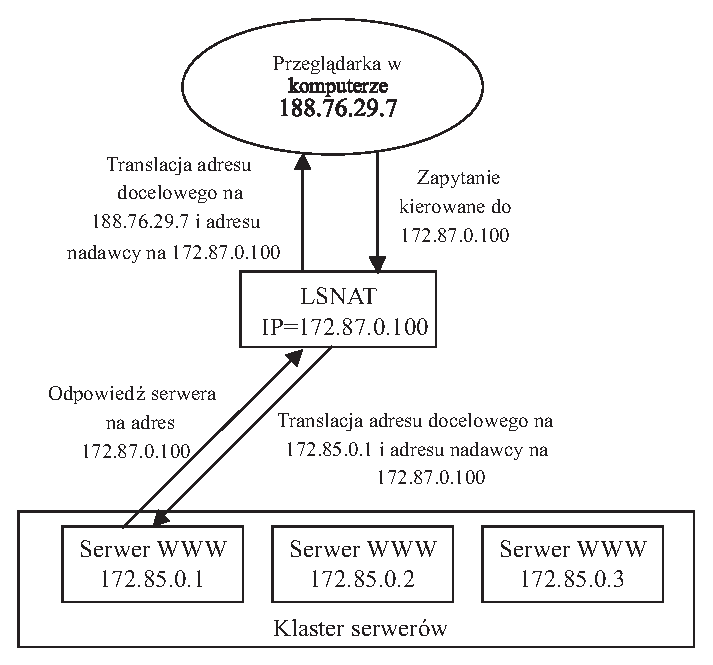
\includegraphics[width=4in]{./rysunki/LocalDirector.eps}
\caption{LSNAT symetrycznie zmieniający adres IP.}
\label{LocalDirector}
\end{figure}

musi więc być instalowany jako jedyne połączenie pomiędzy klasterem a bramką (ang. \emph{gateway}) do sieci rozległej. 
LocalDirector wymaga powielania zawartości pomiędzy serwerami w klastrze. Serwery mogą być połączone z 
LocalDirector-em poprzez sieć Ethernet, FastEthernet lub FDDI. Wybór serwera dokonywany jest sekwencyjnie na 
podstawie wag uwzględniających indywidualne właściwości serwera i jego obciążenie w postaci liczby otwartych 
połączeń TCP. LocalDirector sprawdza czy serwer się nie załamał poprzez okresowe nawiązywanie z nim połączenia 
kontrolnego (Ping, HTTP GET /). Producent zapewnia, że LocalDirector, w zależności od modelu, jest w stanie 
obsłużyć od 7000 do 25000 połączeń na sekundę przy przepustowości od 80 Mbit/sek. do 400 Mbit/sek. Istnieje 
możliwość piętrowej konfiguracji LocalDirector-a. Kilka rozproszonych geograficznie klasterów, z których każdy 
obsługiwany jest przez jedno urządzenie LocalDirector, można zaprezentować jako jeden klaster z użyciem tzw. 
GlobalDirectora. GlobalDirector to w rzeczywistości serwer DNS rozdzielający zapytania pomiędzy klastery na 
zasadzie podobnej do RR--DNS. 

\subsection{F5 Labs BigIP}

BigIP firmy F5 Labs jest tzw. rozwiązaniem ,,pod klucz'' (ang. \emph{turn--key solution}). Oznacza to, że dostarczany 
jest tak jak urządzenie sprzętowe (np. LocalDirector), choć w rzeczywistości jest to komputer pracujący pod 
kontrolą specjalizowanego oprogramowania i systemu operacyjnego firmy F5 Labs. BigIP umożliwia równoważenie 
obciążeń każdego serwera korzystającego z protokołu TCP lub UDP \cite{barylo32,barylo33}. Urządzenie może być podłączone w 
konfiguracji przedstawionej na Rys. \ref{LocalDirector} lub Rys. \ref{LocalDirector1} w obydwu jednak przypadkach, aby uniemożliwić ominięcie 
\begin{figure}[h]
\centering
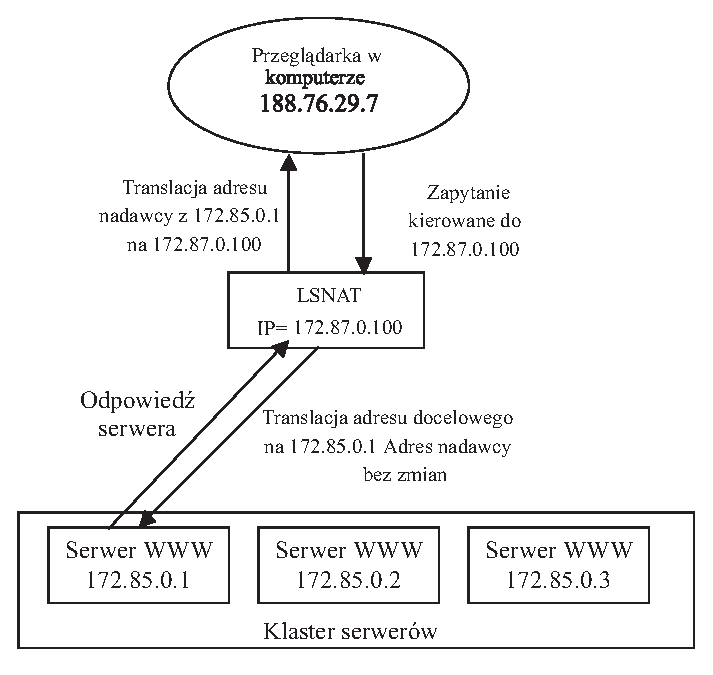
\includegraphics[width=4in]{./rysunki/LocalDirector1.eps}
\caption{LSNAT zmieniający jeden z adresów IP}
\label{LocalDirector1}
\end{figure}

mechanizmu równoważenia obciążeń, BigIP powinien znajdować się pomiędzy klasterem serwerów, a bramką do 
Intetrnet-u. BigIP można połączyć z klasterem poprzez sieć Ethernet, FastEthernet, FDDI lub opcjonalnie 
GigaBitEthernet. Urządzenie oferuje do wyboru siedem algorytmów rozdziału zadań. Trzy z nich to algorytmy 
statyczne, są to: algorytm cykliczny (ang. \emph{Round--robin}); algorytm proporcjonalny przydzielający zadania według 
ustalonych na stałe wag i algorytm priorytetowy, który umożliwia wydzielenie w klastrze grup serwerów o 
określonym priorytecie i rozdział zadań do grup, w każdej z grup serwer do obsługi konkretnego zadania 
wskazywany jest cyklicznie. Pozostałe algorytmy są dynamiczne i uwzględniają obciążenie poszczególnych 
serwerów. Są to algorytm LC (ang. \emph{Least Connections}) przydzielający zadania do serwera utrzymującego najmniej 
otwartych połączeń, algorytm wyznaczający ten serwer, który najszybciej odpowie na zapytanie kontrolne (np. 
HTTP GET /), tzw. algorytm obserwacyjny będący kombinacją powyższych i algorytm predyktywny, który przydziela 
zadania (połączenia) do serwera, którego obciążenie (mierzone jako kombinacja ilości otwartych połączeń i czasu 
odpowiedzi na zapytanie kontrolne) zmniejszało się najszybciej w ciągu np. ostatnich 5 sekund.
Konkretne modele BigIP wyposażone są w procesory Intel Pentium II 450 do 600 MHz pamięć RAM 128 MB do 
1GB i dysk twardy 4 GB do 8.4 GB. Producent gwarantuje przepustowość od 170 Mbit/sek. do 350 Mbit/sek. i 
obsługę do 20000 zapytań na sekundę.
	
\subsection{IBM SecureWay Network Dispatcher}

W związku z tym, że pakiet ten jest jednym z głównych elementów tej pracy, jego dokładny opis i konfiguracja znajduje się 
w następnym rozdziale (Rozdz. \ref{r05}).

